\section{Optimalizace pomocí stochastického gradientního sestupu}
\label{sec:vae_optimization}

Za účelem optimalizace pravé strany \autoref{eq:vae_elbo} je nutné specifikovat tvar, kterého bude $q_\phi(z\mid x)$ nabývat.

Zvolíme $q_\phi(z\mid x) = \mathcal{N}(z\mid \mu(X;\theta),\Sigma(X;\theta))$, kde $\mu$ a $\Sigma$ jsou libovolné \textbf{deterministické} funkce s parametry $\theta$, které se lze učit z dat.
Funkce $\mu$ a $\Sigma$ jsou (typicky) implementovány umělou neuronovou sítí, s tím že $\Sigma$ musí být reprezentována diagonální maticí (viz \autoref{eq:enkoder_diag}).
Takto zvolené $Q(z\mid X)$ má zejména \textbf{výpočetní výhodu} – pravá strana rovnice je nyní jednoznačně spočitatelná. \cite{Doersch2021}

Nyní je tedy poslední prvek pravé strany, $\mathcal{D}_{KL}\left[ Q(z \mid X)\parallel P(z\mid X) \right]$, KL divergence mezi dvěma vícerozměrnými Gaussovými rozděleními.
Takovou KL divergenci lze spočítat v uzavřeném tvaru následovně \cite{Doersch2021}:

\begin{equation}\label{eq:vae_objective_long_form}
    \mathcal{D}_{KL} \left[ \mathcal{N}(\mu(X), \Sigma(X)\parallel \mathcal{N}(0, I)) \right] = 
    \frac{1}{2}\left[ \tr (\Sigma_1^{-1}\Sigma_0) + (\mu_1 - \mu_0)^\top \Sigma_1^{-1}(\mu_1 - \mu_0) - k + \log \left(\frac{\det \Sigma_1}{\det \Sigma_0} \right) \right]
\end{equation}

kde $k$ je dimenzionlita výsledného rozdělení pravděpodobnosti. \autoref{eq:vae_objective_long_form} lze dále zjednodušit následovně \cite{Doersch2021}:

\begin{equation}
    \mathcal{D}_{KL} \left[ \mathcal{N}(\mu(X), \Sigma(X)) \parallel \mathcal{N}(0, I) \right] = 
    \frac{1}{2} \left[ \tr (\Sigma(X)) + (\mu(X))^\top (\mu(X)) - k - \log \det (\Sigma(X)) \right].
\end{equation}

První prvek pravé strany \autoref{eq:vae_elbo} je o něco komplikovanější.

Bylo by možné pomocí vzorků odhadnout $\mathds{E}_{q_\phi(z\mid x^{(i)})} \left[ \log p_\theta(x^{(i)}\mid z) \right]$, ale pro získání \emph{věrohodného} odhadu je nutné skrze $z$ poslat velké množství vzorků, což je výpočetně náročné.
Tedy, jak je u stochastického gradientního sestupu běžné, využijeme pouze jeden vzorek $z$ a použijeme $P(X\mid z)$ pro toto $z$ jako aproximaci této střední hodnoty
\footnote{Zde je výhodou, že provést stochastický gradientní sestup skrze všechny různé hodnoty $X$ vzorkované z datové sady $D$ již stochastický gradientní sestup provádíme při trénování.}. \cite{Doersch2021}


Tedy \textbf{rovnice kterou chceme optimalizovat} má následující podobu \cite{Kingma2014}:

\begin{align}
   \nabla_\phi \mathcal{L}_{\theta,\phi}(x) &= \nabla_\phi \mathds{E}_{q_\phi(z\mid x)} \left[ \log p_\theta (x, z) - \log q_\phi (z\mid x) \right] \label{eq:vae_final_objective} \\
                                            &\neq \mathds{E}_{q_\phi(z\mid x)} \left[ \nabla_\phi (\log p_\theta (x, z) - \log q_\phi (z\mid x) ) \right] \label{eq:vae_final_objective_dependent_gradient}
\end{align}

Symbol gradientu této může být bezpečně přesunut do střední hodnoty.
Tedy, můžeme vzorkovat jednu hodnotu z $X$ a jednu hodnotu ze $z$ z a následně vypočítat gradient \cite{Doersch2021}:

\begin{equation} \label{eq:sample_gradient}
    \log p_\theta(x \mid z) - D_{KL}(q_\phi(\textbf{z}\mid\textbf{x})\parallel p_\theta(\textbf{z})). 
\end{equation}

Průměr gradientu této funkce skrze \emph{libovolně velké} množství vzorků z $x$ a $z$. Výsledná hodnota tohoto gradientu konverguje ke gradientu \autoref{eq:vae_final_objective}. \cite{Doersch2021}

\begin{figure}[H]
    \centering
    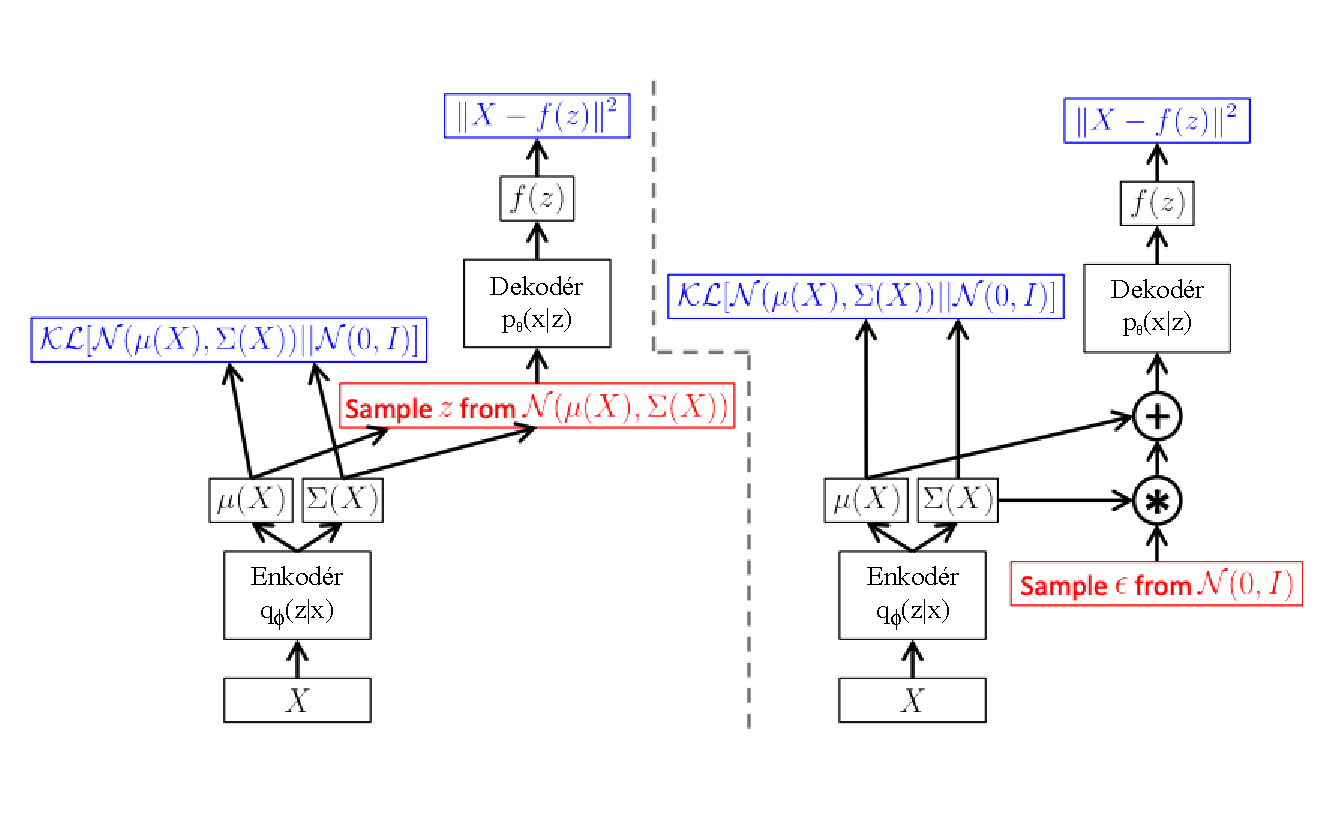
\includegraphics[width=0.95\textwidth]{figures/vae_backpropagation.pdf}
    \caption{Trénovací fáze dopředné umělé neuronové sítě VAE. Levý obrázek je znázorněn bez reparametrizačního triku. Pravý obrázek zahrnuje reparametrizační trik. Červené bloky zobrazují vzorkovací operace, které jsou nediferenciovatelné. Modré bloky zobrazují ztrátové vrstvy neuronové sítě. Dopředné chování obou sítí je \textbf{identické}, ale pouze v síti na pravém obrázku lze provést zpětná propagace. Obrázek včetně interpretace převzat z \cite{Doersch2021}.}
    \label{fig:vae_backpropagation}
\end{figure}

\subsection{Metoda stochastická gradientní optimalizace ELBO}
Důležitou vlastností ELBO je možnost \emph{joint} optimalizace s ohledem na veškeré její parametry – $\boldsymbol{\phi}$ a $\boldsymbol{\theta}$ – za použití stochastického gradientního sestupu (\emph{stochastic gradient descent, SGD}).
Proces lze zahájit náhodnými počátečními hodnotami $\boldsymbol{\phi}$ a $\boldsymbol{\theta}$ a stochasticky optimalizovat jejich hodnoty než dojde ke konvergenci. \cite{Kingma2019}

Mějme nezávisle a rovnoměrně rozdělená vstupní data, účelovou funkcí ELBO je součet ELBO jednotlivých datových bodů \cite{Kingma2019}:
\begin{equation}
    \mathcal{L}_{\theta,\phi}(\mathcal{D}) = \sum_{x\in\mathcal{D}}^{} \mathcal{L}_{\theta,\phi}(\textbf{x})
\end{equation}

ELBO jednotlivých datových bodů a jejich gradienty jsou \emph{obecně} efektivně řešitelné.
Dokonce existují estimátory bez biasu, za pomocí kterých lze provést minibatch SGD.

Gradienty ELBO bez biasu s ohledem na parametry generativního modelu $\boldsymbol{\theta}$ lze jednoduše získat (viz rovnice 2.14 - 2.17 z \cite{Kingma2019}).

Spočítat gradienty ELBO bez biasu s ohledem na variační parametry $\boldsymbol{\phi}$ je již složitější, jelikož tato ELBO je uvažována s ohledem na rozdělení pravděpodobnosti $q_\phi(\textbf{z}\mid\textbf{x})$, tedy je funkcí $\phi$. Nerovnost gradientů ELBO viz rovnice 2.18 - 2.19 z \cite{Kingma2019}.

V případě \textbf{spojitých} latentních proměnných lze využít tzv. \textbf{reparametrizačního triku} pro výpočet odhadů bez biasu $\nabla_{\theta,\phi}\mathcal{L}_{\theta,\phi}(\textbf{x})$.
Tento stochastický odhad umožňuje optimalizovat ELBO za SGD (viz \autoref{alg:reparam_trick})
\footnote{Existují i metody pro případ \textbf{diskrétních} latentních proměnných, které však pro předmět práce nejsou stěžejní. Pro jejich představení odkazuji na \cite[Sekce 2.9.1.]{Kingma2019}.}. Pseudokód algoritmu převzat z \cite{Kingma2019}.

\begin{algorithm}[H]
    \caption{Metoda stochastická gradientní optimalizace ELBO}\label{alg:reparam_trick}
        \KwData{}
                \hspace{6mm}$\mathcal{D}$: Dataset (i. i. d.)\\
                \hspace{6mm}$q_\phi(\textbf{z}\mid\textbf{x})$: Inferenční model (enkodér)\\
                \hspace{6mm}$p_\theta(\textbf{x}, \textbf{z})$: Generativní model (dekodér)\\
        \KwResult{}
        \hspace{6mm}$\boldsymbol{\theta}, \boldsymbol{\phi}$: Naučené parametry\\

        $\boldsymbol{\theta}, \boldsymbol{\phi} \gets \text{Náhodná inicializace parametrů}$

        \While{SGD nezkonvergoval}{
            $\mathcal{M} \sim \mathcal{D}$ (Náhodný \emph{minibatch} vstupních dat)\\
            $\boldsymbol{\epsilon} \sim p(\boldsymbol{\epsilon})$ (Náhodný šum pro každý datový bod v $\mathcal{M}$)\\
            Vypočíst $\tilde{\mathcal{L}}$ and její gradienty $\nabla_{\theta,\phi}(\mathcal{M}, \boldsymbol{\epsilon})$\\
            Upravit $\boldsymbol{\theta}$ a $\boldsymbol{\phi}$ za použití SGD optimizéru
            }
\end{algorithm}

Aby VAE fungovaly dle očekávání, $q_\phi(z\mid x)$ musí být nuceno produkovat takové kódy pro $x$, které bude $p_\theta(x, z)$ schopno \textbf{spolehlivě} dekódovat.
Na tento problém lze alternativně pohlížet interpretací \autoref{eq:vae_final_objective} jakožto sítě, kterou zobrazuje \autoref{fig:vae_backpropagation}(a).
Dopředný průchod této sítě funguje bez problémů – a je-li její výstup zprůměrován skrze mnoho vzorků $x$ a $z$, produkuje správnou střední hodnotu.
Nicméně, je nutné mít schopnost zpětně propagovat chybu skrze vrstvu, která vzorkuje $z$ z $q_\phi(z \mid Xx$, což je \textbf{nespojitá operace} a tedy nemá žádný gradient.
Stochastický gradientní sestup se zpětnou propagací zvládne stochastické vstupy, ale \textbf{neumí pracovat se stochastickými jednotkami (neurony) sítě}.

Řešení tohoto problému nazýváme \textbf{reparametrizační trik}.